\graphicspath{{03-Ckov/Figures/}}

\section{Cherenkov Detectors}
\label{Sect:Ckov}

\subsection{Introduction}
\label{SubSect:Ckov_Intro}
% Lucien Cremaldi (and David Sander) reviewed this

The Cherenkov detectors are primarily designed to provide $\pi$-$\mu$ separation in the higher momentum ranges, where TOF separation is not sufficient for conclusive particle identification.

In order to provide separation over a large range of momenta, two high density silica aerogel Cherenkov detectors (CkovA and CkovB) with refractive indices $n$=1.07 and $n$=1.12 are used.
They are each read out by four 200~mm photomultiplier tubes and placed directly one after another in the beamline, located just after the first TOF counter. In~Fig.~\ref{fig:Ckov} an exploded view of one detector is shown.

Their respective thresholds provide different responses in four distinct momentum ranges, i.e. in the 200 MeV/$c$ beams, pions are below the threshold which would fire the detector for both CkovA and CkovB whereas muons are above only for CkovB, while for the 240 MeV/$c$ beams, pions are above the threshold for CkovB while muons are above for both CkovA and CkovB. Using this information algorithms can be written that produce likelihood distributions of particle type.
Below the CkovB muon threshold of about 217.9~MeV/$c$, where there is no separation, the TOFs provide good separation, whereas the momentum range above the CkovA pion threshold (367.9)~MeV/$c$ is outside of the MICE running parameters~\cite{NOTE473}.
\begin{figure}
  \begin{center}
    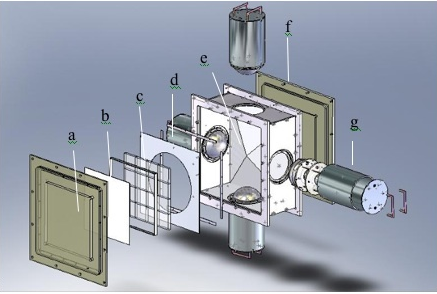
\includegraphics[width=0.6\columnwidth]{./03-Ckov/Figures/Ckov.png}
    \caption{MICE aerogel Cherenkov counter blowup: a)~entrance window, b)~mirror, c)~aerogel mosaic, d)~acetate window, e)~GORE reflector panel, f)~exit window and g)~8~inch PMT in iron shield.}
    \label{fig:Ckov}
  \end{center}
\end{figure}

\subsection{Performance}
\label{SubSect:Ckov_Performance}
